\documentclass{article}
\usepackage[utf8]{inputenc}

\usepackage{biblatex} 
\usepackage{amsmath}
\usepackage{amsfonts}
\usepackage{amssymb}
\usepackage{amsthm}
\usepackage{graphicx}
\usepackage{array}
\usepackage{multirow}
\usepackage{booktabs}
\usepackage{subfig}
\usepackage{mathtools}
\usepackage{bm}
\usepackage{algorithm}
\usepackage{algpseudocode}
\usepackage{dirtytalk}


\usepackage[margin=1.5in]{geometry}


\addbibresource{port.bib}
\bibliography{port.bib}
\usepackage[nottoc]{tocbibind}


\newtheorem{theorem}{Theorem}[section]
\newtheorem{defn}[theorem]{Definition} 
\newtheorem{cor}[theorem]{Corollary}
\newtheorem{alg}[theorem]{Algorithm}
\newtheorem{example}[theorem]{Example}
\newtheorem{lemma}[theorem]{Lemma}
\newtheorem{prop}[theorem]{Proposition}

\setlength{\parskip}{0.5em}

\title{Project Preparation Report}
\author{Hannah Harrison}
\date{April 2023}

\begin{document}

\maketitle

\tableofcontents
\pagebreak

%\section{Planning}

%\begin{enumerate}
%    \item a description of what the problem is (including the current approaches, references to literature and existing methods)
%    \item a high-level description of what you plan to do (obviously you may well not have all the answers yet! But some idea of how you might be tackling it, what the techniques might be, what dataset you might use if appropriate, what balance of theory/simulation of toy data/actual data might be involved and so on)
%    \item a sketch of a plan itself (in terms of the things I discussed on Tuesday - for example, some kind of GANTT chart, timetable or division into work packages and rough schedule, and then also some discussion of risks .. what happens if some of this doesn’t happen as you expect?)
%\end{enumerate}

%2000 ish words

%\pagebreak

\section{Problem Statement and Literature review}

%Reinforcement learning on graphical models

%red and blue agents

%studies on reinforcement 

%XAI problem 

%causal inference. what is a counterfactual etc

%where have people been using causal models 


Given the exponential growth and increased usage of data in the modern world, the need for its protection from theft and damage has become essential. Malicious attacks on cyber networks are becoming increasingly sophisticated and complex. This, combined with the rise in cloud services and the influx of private data from the Internet of Things (IoT) devices, means that the defense scenario is becoming more and more impenetrable. Coordinated attacks can compromise multiple hosts in quick succession once inside a network, necessitating a robust threat detection and response system. 

In \cite{dhir2021prospective}, the authors discuss examples of new malicious tools that current defenders can’t rapidly adapt to, and argue that we need new advanced cyber-defence methods to counter them. They propose the rapid introduction of reinforcement learning (RL) for the purpose of active cyber defence. Indeed, the use of RL techniques in training agents to defend against malicious attacks on networks is gaining popularity, and a large proportion of recent progress in this area is attributable to DeepRL, which utilises deep learning techniques in the training of agents. An up-to-date survey of such techniques is given in \cite{sewak2022deep}, in which the authors emphasise the significant performance improvements DRL techniques have yielded in many complex, real-world security applications. The field of cyber intrusion detection and response is very broad, so I will focus specifically on works which have employed reinforcement learning for automated response. Even within these constraints there have been works showcasing a wide variety of techniques. In \cite{gabirondo2021towards}, the authors utilise a variant of AlphaZero trained using self-play between an attacker and defender agent. Another approach, presented by Hu, Zhu and Liu in \cite{hu2020adaptive}, is to formulate the cyber network as a partially observable Markov Decision Process (MDP) upon which Q-learning is used to find an optimal policy. In \cite{hammar2021learning}, the authors instead try to formulate and solve the problem as an optional stopping problem. Since policies are learned by continually
observing and interacting with the environment, the training of deep RL agents requires large amounts of online data collection, which can be computationally expensive.
One approach to mitigate this is to train in a simulated
environment from which the learned policy can then be shifted to the desired environment with little additional training. Named simulators which have been created to train deep RL agents for cyber threat response are YAWNING TITAN \cite{andrew2022developing}, CyberBattleSim \cite{blum2021gamifying} and CybOrg \cite{standen2021cyborg}. 

Despite the performance enhancements yielded by DeepRL techniques, it is often difficult to explain the decisions made by such agents due to the `black box' nature of many deep learning methods \cite{PearlMackenzie18}. This lack of explainability can make algorithms difficult to trust, understand and verify, yielding both ethical and practical concerns. Such problems are highlighted when an agent behaves in an unpredictable manner, which can occur when the target environment is outside of the `training bounds' of the agent, i.e. when the target environment is significantly different to the environment in which the agent was trained. This problem causes significant concern in highly dynamic domains such as the defense of cyber networks, in which the environment and attack vectors are prone to change quickly and frequently. Further, the use of simulations to develop deep RL agents as mentioned above can also cause the training and target environments to differ. Hence an improvement in the explainability of deep RL agents could help in the understanding and predictability of the algorithm's behaviour. Moreover, deep RL models are complex to debug \cite{heuillet2021explainability}, and an explainable model could aid in fixing problems more quickly and accelerate new development in RL methods. 

The emerging area of research which focuses on explaining the decisions of RL agents has been coined Explainable Reinforcement Learning (XRL) and is a relatively new subfield of Explainable AI (XAI) research. Much progress in XRL has been achieved by making use of existing XAI methods \cite{wang2022causal}, and in particular \cite{heuillet2021explainability} provides a review of recent developments in XAI and makes suggestions on how these techniques may be adapted to deep RL policies. For example, some XRL techniques stem from the XAI saliency map method \cite{simonyan2013deep} which provides explanations for image classification by identifying `important' pixels. In turn, some XRL methods attempt to provide explanations by generating maps that identify `important' state features, for example \cite{greydanus2018visualizing}. However, most of these studies take an associational perspective; `importance' is measured in terms of the correlation between state features and the subsequent action. As follows from the commonly accepted notion that \say{Correlation does not imply causation} (\cite{PearlMackenzie18}), features which are highly correlated with a given action may not actually be real `causes', resulting in incorrect explanations. This can degrade trust in the system.


Many researchers in the field of XAI argue that `better' explanations (in terms of human understandability and reliability) can be extracted from models by considering causality \cite{madumal2020explainable}. While a majority of machine learning models focus on correlations found between features in the training data, these correlations can be coincidental and what we are actually interested in is the causal effect of one variable on another \cite{PearlMackenzie18}. The branch of science devoted to understanding such causal relationships is known as causality, and it is widely accepted that human cognition and understanding relies on such relationships, hence the notion that causal models generate explanations which are easier for humans to understand. This idea is explored for explaining the decisions of an RL agent in \cite{madumal2020distal}, where the authors perform human experiments to compare explanations for an RL agent's decisions in the context of the video game Starcraft II. In particular, the explanations yielding the highest scores in terms of understanding and user satisfaction utilised counterfactuals; outcomes which were not observed but could have occured under different circumstances. Hence, causal models can help to provide explanations which emulate human retrospective thinking, aiding the understanding of RL models. Another relevant work on the topic of XRL is \cite{wang2022causal}, in which the authors develop a causal explanation mechanism for Markovian policies that quantifies causal importance of states on actions over time. In particular, a causal model is used to provide insight into which factors most heavily influence an agent's decision at a given time. The authors also demonstrate via simulation the advantage of their causal method over explanations generated using associational methods. Such methods have the potential to improve the reliability and trust in the information available to humans making time-critical cyber-defense decisions. 

The main aim of this research is to explore the application of causal models to explain the decisions made by deep RL
agents in the context of cyber threat response.



\pagebreak

\section{Project Proposal}

%a high-level description of what you plan to do (obviously you may well not have all the answers yet! But some idea of how you might be tackling it, what the techniques might be, what dataset you might use if appropriate, what balance of theory/simulation of toy data/actual data might be involved and so on)

\subsection{Project aims}
As suggested in the project brief, I plan to divide the research into three main strands. In particular, I aim to:
\begin{enumerate}
    \item Explore the use of reinforcement learning in simulated networks and develop a reinforcement learner which can defend against simple attacks.
    \item Survey the application of causal models for the purpose of providing explanations for reinforcement learning.
    \item Develop a proof of concept which utilises a causal model to explain the decisions made by the reinforcement learner I developed in Part 1. 
\end{enumerate}

\noindent This project will be heavily simulation based, and the reinforcement learner developed will aim to identify the best action to take in order to limit the spread of an intrusion through a simulated network. The focus of the project is not to develop the most effective reinforcement learner, but to develop one for which it will be possible to explain the decisions made. However, in order to yield a realistic result, the reinforcement learner should meet some basic standard of performance, which will need to be decided upon in advance through research into existing performance metrics. I aim to develop a very flexible reinforcement learner and so I will vary the configuration of the simulated network in order to test the policies in different settings. As mentioned in Section 1, there exists a large body of research into the use of deep RL in cyber threat detection and response, and so an initial task will be to survey this research, and experiment with different techniques. A particularly useful resource will be \cite{sewak2022deep}, which reviews deep reinforcement learning techniques within the cybersecurity field. While the context is fairly broad, the authors provide useful explanations about the differences between types of reinforcement learning (such as policy based versus value based approaches) which may aid in selecting appropriate approaches for my setting. 

Following the development of the reinforcement learner, I will move on to reviewing the literature on causal models, with particular emphasis on their application to explaining the decisions made by RL agents. A useful starting point will be \cite{heuillet2021explainability}, a 2021 review of XRL literature. In particular, Table 3 provides a list of XRL papers along with the task environment, RL algorithm used and explanation type, providing a useful overview of the techniques I can investigate. Further, \cite{heuillet2021explainability} also provides guidelines on evaluating explanations which will be useful when considering the effectiveness of causal explanation mechanisms. 

\subsection{Methods and tools}
The primary tool I will be using in this project is YAWNING TITAN \cite{andrew2022developing}, an abstract graph-based cyber simulator. 
In particular, YAWNING TITAN models real-world computer networks to predict the outcomes of actions taken by red and blue agents. YAWNING TITAN is a relatively recent construction (released in July 2022) and was built for the purpose of training intelligent agents in cyber defense situations \cite{andrew2022developing}. The advantage of YAWNING TITAN is that it is highly flexible and abstract, requiring little specific network information, and so should be ideal for developing a RL policy which performs well on a variety of networks. The simulator is built for use in Python, so I will be able to apply my existing programming skills in this project. 

YAWNING TITAN has the inbuilt capability to produce visualisations of the current episode, an example of such is shown in Figure \ref{fig:YT}. This illustrates the setup of the training scenarios, with red indicating the path of the attacker and blue representing the path of the `blue agent'. In particular, the goal of the blue agent is to block the path of the attacker and prevent the compromise of further nodes. Hence the goal of my reinforcement learner will be to select actions which minimise the spread of compromised nodes based on the information available, in particular the `known compromises' shown circled in blue on Figure \ref{fig:YT}. The visualisation capabilities of YAWNING TITAN will aid me in understanding the state of the network when the agent makes each decision, and hence will aid in evaluating the explanations of these actions produced by causal mechanisms in the final stage of the project. 

Figure \ref{fig:YT} also indicates how YAWNING TITAN enables the user to set differing node vulnerability scores, and select high value nodes in order to better reflect real networks. 

\begin{figure}[htp]
    \centering
    \includegraphics[width=0.99\textwidth]{Images/YT example.png}
    \caption{An example network situation produced within the YAWNING TITAN environment \footnotemark .}
    \label{fig:YT}
\end{figure}

\medskip
\medskip
\medskip
\medskip
\medskip
\medskip
\medskip



\footnotetext{Image taken from \cite{YTexample}.}

\section{Timeline}

\subsection{Gantt Chart}
Figure \ref{fig:gantt} displays a Gantt chart proposing a timeline for the project workload. Much of the initial work will focus on exploring YAWNING TITAN in order to better understand its capabilities, as it is a relatively new construction and little documentation exists of its usage. During this time I will also survey existing work on deep RL techniques and identify the most appropriate to implement. Next, I plan to begin reviewing applications of causal modelling in the generation of explanations for RL policies. I envision a large part of the final report being devoted to this survey of current research, and so I allocated around a month to this task, and will begin writing these findings up as I go along. I will also synchronously experiment with implementing the causal modelling techniques I find, before beginning the final stage of the project; the development of a causal explanation mechanism for my reinforcement learner. 

\begin{figure}[htp]
    \centering
    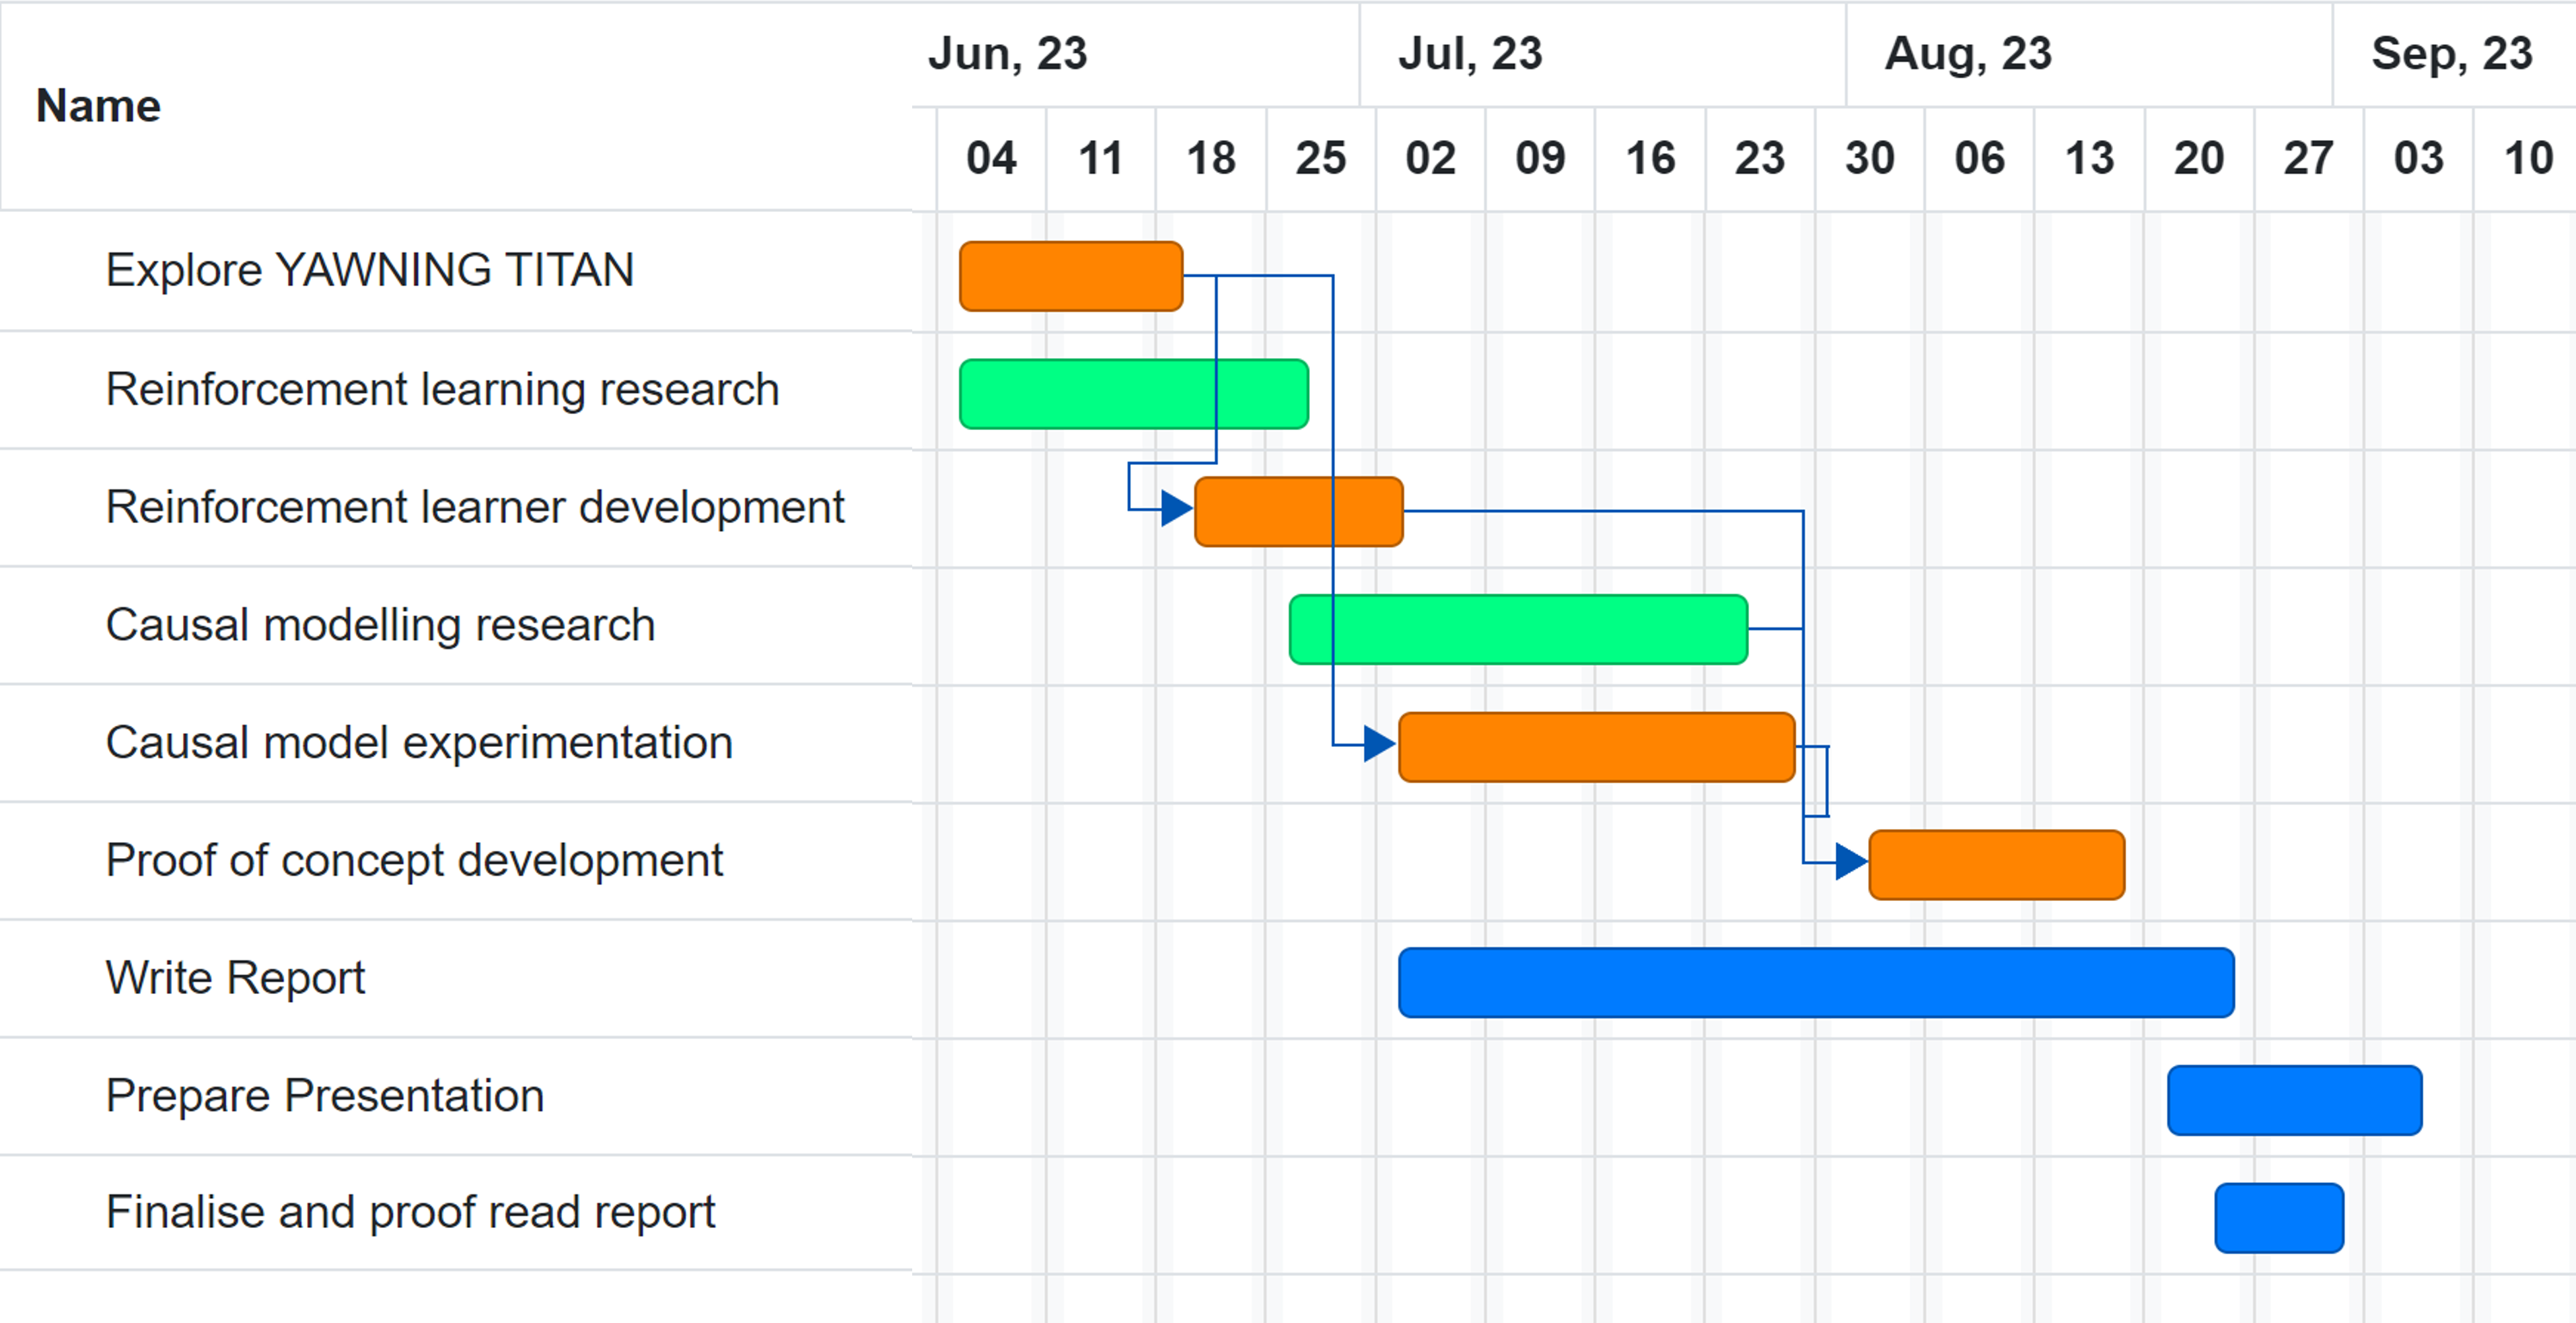
\includegraphics[width=0.99\textwidth]{Images/gantt.png}
    \caption{Gantt chat breaking down the project workload. Programming tasks are shown in orange, research tasks in green and writing tasks in blue. The arrows represent dependencies between tasks.}
    \label{fig:gantt}
\end{figure}


%timeline and gantt chart 

\subsection{Potential problems}
%contingency plans for if yawning titan has problems. Include plan b options 

The greatest potential complication is experiencing issues with YAWNING TITAN.  In particular, as it is relatively new and I have thus far found little documentation of its use, I may not be able to use all of its capabilities, or indeed it may not be possible to implement the reinforcement learning or causal modelling techniques I find on the networks generated. 

As shown by the task dependencies in the Gantt chart (represented by arrows), learning how to use the cyber simulator is essential to the project progress, as I can't begin to implement reinforcement learning nor the subsequent causal models until I have a working simulated network. Thus the focus of the first few weeks of my project will be to investigate YAWNING TITAN and this will aid in understanding how I can best use it. If indeed it does turn out to be difficult to use and the reinforcement learners difficult to implement, then I will spend up to an additional two weeks on this exploration. As is evident on the Gantt chart, this comes with little consequence on the progress of the rest of the project, as the reinforcement learner research is a deliverable on its own. If after these additional weeks YAWNING TITAN still seems unusable,
then I will consider other cyber simulators available. A useful resource for this will be Section 3 of \cite{andrew2022developing}, as the authors compare cyber simulators used in other works related to selecting optimal defensive actions in a network. In particular, a promising potential alterantive is Microsoft's Cyber Battle Simulator \cite{blum2021gamifying}. Whilst this switch would lose some of the abstraction offered by YAWNING TITAN (in particular the Cyber Battle Simulator requires host information
such as specific host vulnerabilities and an in-depth environment
setup), the simulator is still very flexible and should allow for similar experimentation. Like YAWNING TITAN, CyberBattleSim is also built using a Python-based Open AI Gym interface, resulting in less lost work if I do need to switch between the two simulators. Further, although Cyber Battle Simulator is also a very new development (released in 2021), the github repository \cite{msft:cyberbattlesim} is very active, suggesting a good level of support for the project. 


Another potential issue I could face in this project is that the development of the reinforcement learner could take longer than expected, delaying the rest of the project as this is a key dependency for the development of the causal explanation mechanism. If this is the case, I plan to still begin researching causal model implementations alongside working on the reinforcement learning, and if short on time I will modify the project to give a survey of current research and intuition on how other applications of causal modelling in explaining  reinforcement learning could be applied and extended in the context of cyber threat response. Likewise, the contingency plan in the case that I simply fail to produce a working proof of concept is to explain the limitations of the methods I tried and give intuition on why they weren't applicable. 

Table \ref{tab:comparison} gives a summary of the key project milestones and the contingency plans discussed for easy reference.

\begin{table}[h!]
    \centering
    \small
    \begin{tabular}{ | m{0.3\textwidth} | m{0.2\textwidth} |m{0.4\textwidth} |} 
      \hline
       Milestone & Date & Contingency plan if missed \\ 
      \hline
       YAWNING TITAN toy model working & 18/06/23 & Spend up to an additional two weeks on task. If not complete by 30/06/23 then consider alternative simulators. \\ 
      \hline
       Reinforcement learner developed & 02/07/23 & Spend additional time on the task. Begin causal modelling research as planned and consider giving suggestions for causal mechanisms rather than proof of concept if short on time. \\ 
      \hline
      Working proof of concept & 20/08/23 & Leave project here. Focus on explaining limitations of methods tried and why they didn't work. \\ 
      \hline
      
    \end{tabular}
    \caption{Summary of project milestones and plans for if they are missed.}
    \label{tab:comparison}
\end{table}

\pagebreak



\section{References}

\printbibliography[heading=none, stylename = plain]

\end{document}
